\chapter{Fundamentação Teórica}
\label{c.fundamentacaoteorica}

Em Ciência da Computação, compressão de dados é o processo de codificar as mesmas informações usando um número menor de bits, sem que haja distorção dos dados originais. Em se tratando de compressão de imagens, pode-se alcançar Esse processo é útil, pois reduz o consumo de recursos computacionais, como espaço em disco, ou utilização de banda de internet.

Considere as imagens abaixo.

\begin{figure}[h]
\caption{\small Codificador e Decodificado de Imagens}
\centering
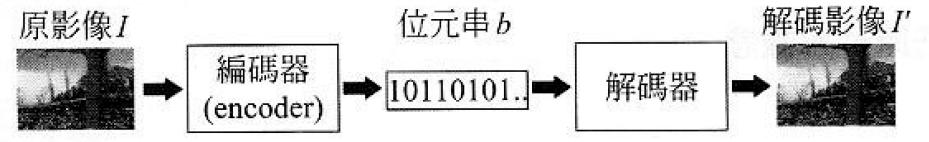
\includegraphics[scale=0.50]{figs/image_compression.jpg}
\label{f.imagecompressionbasics}
\legend{\small Fonte: Elaborada pelo autor.}
\end{figure}

Quando o sistema recebe a imagem original, ele manda para um codificador que converte a imagem original para um fluxo de bits. Um decodificador então recebe esse fluxo de bits e o transforma novamente na imagem. Caso o fluxo de bits final seja menor que o original, chamamos esse processo de Compressão de Imagem.



\section{Métodos de Compressão}
\label{s.metodos}



De acordo com \citeauthoronline{hackerdictionary} (\citeyear{hackerdictionary}) define um {\em hacker} como sendo uma pessoa que contenha as seguinte características:

\begin{alineas}
  \item Uma pessoa a qual aprecia aprender detalhes de uma linguagem de programação ou de um sistema;
  \item Uma pessoa a qual aprecia programar ao invés de apenas teorizar;
  \item Uma pessoa capaz de apreciar o {\em hackeamento} de outra pessoa;
  \item Uma pessoa que aprende rapidamente uma linguagem de programação;
  \item Uma pessoa que é perito em determinada linguagem de programação ou sistema computacional.
\end{alineas}



\section{Algoritmos}
\label{s.algoritmos }



\begin{alineas}
  \item Recolher informações do alvo, antes do teste (reconhecimento);
  \item Identificar possíveis pontos de entrada;
  \item Tentativa de invasão, seja virtualmente ou pessoalmente;
  \item Reportar as descobertas.
\end{alineas}



\subsection{Por que realizar Testes de Penetração?}
\label{ss.whypentest}



\citeauthoronline{pentestbefore} cita que o motivo principal para realização de Testes de Penetração é de encontrar vulnerabilidades através de ganho de acesso e resolver estas falhas. Porém, além desse motivo principal, também é citado que é uma boa prática ter o sistema verificado por olhos que não estavam inicialmente no projeto, podendo assim encontrar falhas não verificadas anteriormente. Outros motivos que são citados, podemos listar os seguintes:

\subsection{Estágios de um Teste de Penetração}
\label{ss.stagespentest}


% \subsection{Teste de Penetração como Área Forense}
% \label{s.pentestforense}

\section{Computação na Nuvem}
\label{s.cloudcomputing}

Dentre os diversos benefícios que a Computação na Nuvem trás, podemos listar:

\begin{alineas}
  \item Os recursos oferecidos suprem a maioria das demandas de quase todos os ramos de empresas;
  \item Elasticidade, ou seja, o poder de aumentar ou diminuir os recursos, conforme se é necessário;
  \item Pagar somente pelos recursos que são utilizados.
\end{alineas}

\subsection{Tipos de Serviços na Nuvem}
\label{s.cloudservices}

Segundo \citeauthoronline{clouddefinition}, em '{\em A comprehensive look at the path to cloud migrations}', Serviços de Computação na Nuvem são divididos nos seguintes tipos:
